\documentclass[serif]{beamer}

\renewcommand\sfdefault{phv}
\renewcommand\familydefault{\sfdefault}
\usetheme{default}
\usepackage{color}
\usepackage{verbatim}
%\usepackage{pxfonts} % Or palatino or mathpazo
%\usepackage{eulervm}
\useoutertheme{default}
%\usepackage{texnansi}
\usepackage{color}
%\usepackage{marvosym}
\definecolor{bottomcolour}{rgb}{0.32,0.3,0.38}
\definecolor{middlecolour}{rgb}{0.08,0.08,0.16}
\setbeamerfont{title}{size=\Huge}
\setbeamercolor{structure}{fg=gray}
\setbeamertemplate{frametitle}[default]%[center]
%\setbeamercolor{normal text}{bg=black, fg=white}
%\setbeamertemplate{background canvas}[vertical shading]
%[bottom=bottomcolour, middle=middlecolour, top=black]
\setbeamertemplate{items}[circle]
\setbeamerfont{frametitle}{size=\huge}
\setbeamertemplate{navigation symbols}{} %no nav symbols
\usefonttheme[stillsansseriflarge]{serif}

\usepackage{amsmath,  amsfonts, amsthm, graphicx, subfigure}
%\usepackage{biblatex}
 \usepackage{fancybox, ulem}
 \usepackage{mathtools}
 \usepackage{tabularx}
 \usepackage{tikz}
 \usepackage{movie15}
 %\bibliography{pumping_paper}
\newcommand{\p}{\partial}
\newcommand{\f}{\frac}
\newcommand{\B}{\textbf}
\newcommand{\I}{\textit}
\newcommand{\tab}{\hspace{10mm}}

 % \usetheme{Singapore}
% \usetheme{Warsaw}
  \setbeamertemplate{navigation symbols}{}
\title{Lecture 11}
\author{Austin Baird\\UNC Department of Mathematics\\UNC Department of Biology}
\date{\today} 

\begin{document}
\frame{\titlepage}

\begin{frame}
\frametitle{Summary}

Today we will: 
\ \\
\ \\
Try and understand series approximations and transforms (\textcolor{red}{Fourier Analysis!}) 
\end{frame}

%--------------------------------------------------------------------------------------------------------------------------------------------------------------------------------------------------------------------------%
\begin{frame}
\frametitle{Periodic Functions}

A period function satisfies the relationship: 

\begin{align*}
f(t+nP) &= f(t)\\
n &\in \mathcal{Z}
\end{align*}

Here the period is denoted $P$ and so this relations shows that for any chosen $n$ the graph will repeat itself with period $P$. Think of reconstructing a graph to have as large of a domain as you'd like by reflecting a function over and over again about the period!


\end{frame}
%%%%--------------------------------------------------------------------------------------------------------------------------------------------------------------------------------------------------------------------------%

\begin{frame}

\frametitle{Series Expansion of Periodic Functions} 

Sometimes, \textcolor{red}{Periodic} functions can be written as an infinite series of $\sin$ and $\cos$'s. This can be referred to as the \textcolor{red}{Fourier series} of a function: 

\begin{align*}
f(x) = \frac{a_0}{2} + \sum^{\infty}_{n=1}[a_n\cos\left(\frac{n\pi x}{L}\right) + b_n\sin\left(\frac{n\pi x}{L}\right)]
\end{align*}

Here our coefficients $a_n$ and $b_n$ can be written as: 

\begin{align*}
a_n &= \frac{1}{L} \int^{L}_{-L} f(x)\cos \left(\frac{n\pi x}{L}\right) dx \\
b_n &= \frac{1}{L} \int^{L}_{-L} f(x)\sin \left(\frac{n\pi x}{L}\right) dx 
\end{align*}

\end{frame}


%%%%--------------------------------------------------------------------------------------------------------------------------------------------------------------------------------------------------------------------------%
%%

\begin{frame}
\frametitle{Let's Try It!} 

Find the Fourier series of the \textcolor{red}{sawtooth} function: 

\begin{align*}
&f(x) = x \; \; \;  -L < x < L \\
&f(x+2L) = f(x)
\end{align*}


Now we want to graphically show that if we truncate this series it gives a good approximation.  \textcolor{red}{Do It!} 

\pause

\begin{align*}
a_n &= \frac{1}{L} \int^{L}_{-L} f(x)\cos \left(\frac{n\pi x}{L}\right) dx = 0 \;\;\; n=0,1,2\hdots \\
b_n &= \frac{1}{L} \int^{L}_{-L} f(x)\sin \left(\frac{n\pi x}{L}\right) dx  = \frac{-2L}{n\pi}(-1)^n \;\;\; n=1,2,3\hdots
\end{align*}


\end{frame}
%%%%--------------------------------------------------------------------------------------------------------------------------------------------------------------------------------------------------------------------------%

\begin{frame}
\frametitle{Example Continued} 

We now have a full formula for the series of our sawtooth function: 

\begin{align*}
f(x) =\sum^{\infty}_{n=1}\left[ \frac{-2L}{n\pi}(-1)^n\sin\left(\frac{n\pi x}{L}\right)\right]
\end{align*}

This function is an \textcolor{red}{exact} approximation to our function except at the discontinuities! 

\end{frame}
%%%%--------------------------------------------------------------------------------------------------------------------------------------------------------------------------------------------------------------------------%

\begin{frame}
\frametitle{Comparison}

Sampling a finite number of series terms we can get a pretty good representation: 

\begin{figure}
\includegraphics[width=\textwidth,height=0.7\textheight]{./sawtooth}
\end{figure}

\end{frame}

%%%%--------------------------------------------------------------------------------------------------------------------------------------------------------------------------------------------------------------------------%


\begin{frame}
\frametitle{Fourier Integral Representation}

Unfortunately the fourier series representation of a function only works for \textcolor{red}{periodic} functions, what about \textcolor{red}{non-periodic} functions? For this we use the \textcolor{red}{Fourier integral} representation: 


\begin{align*}
f(x) &= \int^{\infty}_{0} a(k) \cos(kx)dk + \int^{\infty}_0 b(k) \sin (kx)dk\\
a(k) &= \frac{1}{\pi}\int^{\infty}_{\infty}f(x)\cos (kx) dx\\
b(k) &= \frac{1}{\pi}\int^{\infty}_{\infty}f(x)\sin (kx) dx
\end{align*}

This definition now has a continuous frequency resolution and is defined for non-period functions defined on $(-\infty,\infty)$
\end{frame}

%
%%%%%--------------------------------------------------------------------------------------------------------------------------------------------------------------------------------------------------------------------------%
%
\begin{frame}
\frametitle{Fourier transform!}
We can now write this representation using a singular integral and using \textcolor{red}{Eulers equation:} $ e^{i\theta} = \cos(\theta) + i\sin{\theta}$. 

\begin{align*}
\hat{f}(k) = \frac{1}{\sqrt{2\pi}}\int^{\infty}_{\infty}f(x)e^{-2\pi i x k}dx
\end{align*}

With an inverse defined to be: 


\begin{align*}
f(x) = \frac{1}{\sqrt{2\pi}}\ \int^{\infty}_{\infty}\hat{f}(k)e^{2\pi i x k}dk
\end{align*}

Similarly we could transform a function defined with time ($t$). Also note that $k$ is the frequency of the function. 

\end{frame}
%%%%--------------------------------------------------------------------------------------------------------------------------------------------------------------------------------------------------------------------------%


\begin{frame}
\frametitle{Discrete Transform} 

Now assume that we aren't transforming a function but a sequence of data, $\{f_{k}\}_{k=0}^{N-1}$ which we know contains some oscillations: (sample the sin wave) we get: 


\begin{align*}
\hat{F}_n = \sum_{n = 0}^{N-1}f_ke^{\frac{-2\pi i k n}{N-1}}
\end{align*}
Here $\hat{F}_n$ is the Fourier transform of the data $f_k$ sampled at $N$ data points. Here $k$ is the frequency. Note that $\hat{F}_n$ is a sequence of numbers: $n = 0,1,\hdots N-1$ which is the same size as the number of times we sampled the data: $f_k$\\

\textcolor{red}{Note:} We cannot compute zero or negative indices in matlab, so we will shift this formula by 1: 

\begin{align*}
\hat{F}_n = \sum_{n = 1}^{N}f_ke^{\frac{-2\pi i (k-1) (n-1)}{N-1}}
\end{align*}

\end{frame}

%%%%--------------------------------------------------------------------------------------------------------------------------------------------------------------------------------------------------------------------------%

\begin{frame}
\frametitle{Discrete Transform}

Turns out we can write this as matrix vector multiplication! If we define an $NxN$ matrix for $\omega_n = e^{\frac{-2\pi i}{n}}$ we can define it to be: 

\begin{align*}
\begin{pmatrix}
F_0\\
F_1\\
\vdots\\
F_{n-1}
\end{pmatrix}
=
\begin{pmatrix}
1 & 1 & \hdots & 1\\
1 & \omega^{1\cdot 1}_{n} &\hdots &  \omega^{1\cdot (n-1)}_{n}\\
 \vdots & \vdots & \ddots & \vdots\\
 1 &  \omega^{(n-1) \cdot 1}_{n} & \hdots &  \omega^{(n-1)\cdot (n-1)}_{n} 
 \end{pmatrix}
 \begin{pmatrix}
 f(x_0)\\
 f(x_1)\\
 \vdots\\
 f(x_{n-1})
 \end{pmatrix}
\end{align*}

Now we have what we need to get $[F_n]$. Since we know $f_k$, sampled data, and we can compute the matrix! 
\end{frame}
%%%%--------------------------------------------------------------------------------------------------------------------------------------------------------------------------------------------------------------------------%

\begin{frame}
\frametitle{Fast Fourier Transform} 

So what is wrong with what we just computed? \textcolor{red}{Computational Cost!} To compute this directly = $\mathcal{O}(n^2)$, but there is a new way! \textcolor{red}{FFT!}
Idea: \\
\ \\
\ \\
\begin{itemize}
\item  Use symmetry of the matrix to compute the multiplication without recomputing matrix terms! 
 \item Speeds up computational time to $\mathcal{O}(n\log(n))$ 
 \end{itemize}

\end{frame}

%%%%--------------------------------------------------------------------------------------------------------------------------------------------------------------------------------------------------------------------------%

\begin{frame}
\frametitle{Examples} 

Periodic data = frequency analysis: 

\begin{figure}[h]
\includegraphics[width=\textwidth,height=0.7\textheight]{./freq}
\end{figure}
 
 \textcolor{red}{But how do we get the frequency!?}

\end{frame}

%
%%%%%%--------------------------------------------------------------------------------------------------------------------------------------------------------------------------------------------------------------------------%
\begin{frame}[fragile]
\frametitle{Frequency}
To get the frequency spectrum of the data you are analyzing, do the following (in Matlab) :
\ \\
\begin{verbatim}
Fs = 150;    sampling frequency 
t = 0:1/Fs:1;    discretized time domain
f = 5;    frequency of our sin wave
y = sin(2*pi*f*t);
nfft = 1024;    length of the fft domain, power of 2 
x = fft(y,nfft);
x = abs(x(1:nfft/2)); Half of the data, fft is symmetric
f = (0:nfft/2-1)*Fs/nfft;    frequency vector
\end{verbatim}

\end{frame}
%%%%%%--------------------------------------------------------------------------------------------------------------------------------------------------------------------------------------------------------------------------%

\begin{frame}
\frametitle{Homework 10}

We want to gain an understanding of Fouier analysis a variety of ways: 

\begin{itemize}
\item Compute the series expansion for the top hat periodic function: 
\end{itemize}
\begin{align*}
f(x) &= \left\{
\begin{array}{l l}
-1& \quad -1<x < 0 \\
1 & \quad 0\leq x <1 
\end{array}
 \right.\\
 f(x+2) &= f(x) \quad  \textrm{(periodic condition)}
 \end{align*}

Graph the actual function and the series representation truncated at the first 2,4,8,10 terms. 
\end{frame}
%
%%%%%--------------------------------------------------------------------------------------------------------------------------------------------------------------------------------------------------------------------------%
\begin{frame}

\frametitle{Homework 10}

\begin{itemize}
\item Program the Discrete Fourier transform for a periodic function and compute it's frequency. 
\item Use the periodic function $f(t) = sin(2\pi 50 t) + sin(2\pi120 t)$ in your computations (it has what frequencies?) 
\item Vary the number of sampling points and test the time it takes to compute.
\begin{itemize}
\item  Let sampling be power of 2 and compute the time it takes to compute the problem (graph the data x-axis = sample points, y-axis = compute time)
\item Watch this movie: \url{http://blogs.mathworks.com/pick/2008/02/12/timing-code-in-matlab/}, it will help you! 
\end{itemize}
\end{itemize}

\end{frame}

\begin{frame}
\frametitle{This is what it should look like} 

\begin{figure}
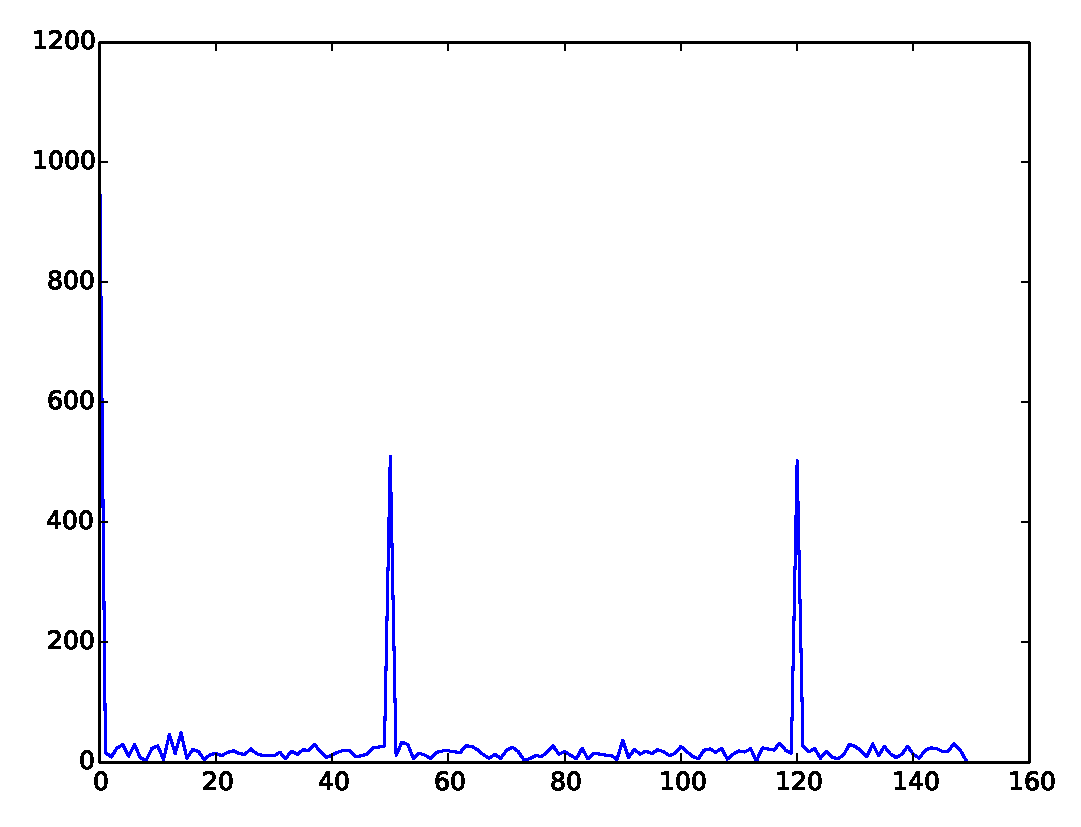
\includegraphics[width=\textwidth,height=0.8\textheight]{./freq_hw}
\end{figure}

\end{frame}
%%%%--------------------------------------------------------------------------------------------------------------------------------------------------------------------------------------------------------------------------%
%

\begin{frame}
\frametitle{Homework 10}

\begin{itemize}

\item Use the data provided 
\item The data is a loaded elastic material extended into a sin wave, immersed into a fluid. The deformed boundary is released and then vibrates to rest. 
\item Goal: Extract the frequency of the vibrating boundary! 
\begin{itemize}
\item Load it into matlab 
\item make a graph of it over time ( it contains two columns, position and time)
\item Take an fft of the data
\item Graph the frequency spectrum
\item Explain issues and why there are several predominant frequencies.
\end{itemize}
\end{itemize}
\end{frame}

%%%%%--------------------------------------------------------------------------------------------------------------------------------------------------------------------------------------------------------------------------%
%

\end{document}
